% Options for packages loaded elsewhere
% Options for packages loaded elsewhere
\PassOptionsToPackage{unicode}{hyperref}
\PassOptionsToPackage{hyphens}{url}
%
\documentclass[
  english,
  russian,
  12pt,
  a4paper,
  DIV=11,
  numbers=noendperiod]{scrreprt}
\usepackage{xcolor}
\usepackage{amsmath,amssymb}
\setcounter{secnumdepth}{5}
\usepackage{iftex}
\ifPDFTeX
  \usepackage[T1]{fontenc}
  \usepackage[utf8]{inputenc}
  \usepackage{textcomp} % provide euro and other symbols
\else % if luatex or xetex
  \usepackage{unicode-math} % this also loads fontspec
  \defaultfontfeatures{Scale=MatchLowercase}
  \defaultfontfeatures[\rmfamily]{Ligatures=TeX,Scale=1}
\fi
\usepackage{lmodern}
\ifPDFTeX\else
  % xetex/luatex font selection
\fi
% Use upquote if available, for straight quotes in verbatim environments
\IfFileExists{upquote.sty}{\usepackage{upquote}}{}
\IfFileExists{microtype.sty}{% use microtype if available
  \usepackage[]{microtype}
  \UseMicrotypeSet[protrusion]{basicmath} % disable protrusion for tt fonts
}{}
\usepackage{setspace}
% Make \paragraph and \subparagraph free-standing
\makeatletter
\ifx\paragraph\undefined\else
  \let\oldparagraph\paragraph
  \renewcommand{\paragraph}{
    \@ifstar
      \xxxParagraphStar
      \xxxParagraphNoStar
  }
  \newcommand{\xxxParagraphStar}[1]{\oldparagraph*{#1}\mbox{}}
  \newcommand{\xxxParagraphNoStar}[1]{\oldparagraph{#1}\mbox{}}
\fi
\ifx\subparagraph\undefined\else
  \let\oldsubparagraph\subparagraph
  \renewcommand{\subparagraph}{
    \@ifstar
      \xxxSubParagraphStar
      \xxxSubParagraphNoStar
  }
  \newcommand{\xxxSubParagraphStar}[1]{\oldsubparagraph*{#1}\mbox{}}
  \newcommand{\xxxSubParagraphNoStar}[1]{\oldsubparagraph{#1}\mbox{}}
\fi
\makeatother


\usepackage{longtable,booktabs,array}
\usepackage{calc} % for calculating minipage widths
% Correct order of tables after \paragraph or \subparagraph
\usepackage{etoolbox}
\makeatletter
\patchcmd\longtable{\par}{\if@noskipsec\mbox{}\fi\par}{}{}
\makeatother
% Allow footnotes in longtable head/foot
\IfFileExists{footnotehyper.sty}{\usepackage{footnotehyper}}{\usepackage{footnote}}
\makesavenoteenv{longtable}
\usepackage{graphicx}
\makeatletter
\newsavebox\pandoc@box
\newcommand*\pandocbounded[1]{% scales image to fit in text height/width
  \sbox\pandoc@box{#1}%
  \Gscale@div\@tempa{\textheight}{\dimexpr\ht\pandoc@box+\dp\pandoc@box\relax}%
  \Gscale@div\@tempb{\linewidth}{\wd\pandoc@box}%
  \ifdim\@tempb\p@<\@tempa\p@\let\@tempa\@tempb\fi% select the smaller of both
  \ifdim\@tempa\p@<\p@\scalebox{\@tempa}{\usebox\pandoc@box}%
  \else\usebox{\pandoc@box}%
  \fi%
}
% Set default figure placement to htbp
\def\fps@figure{htbp}
\makeatother



\ifLuaTeX
\usepackage[bidi=basic,provide=*]{babel}
\else
\usepackage[bidi=default,provide=*]{babel}
\fi
% get rid of language-specific shorthands (see #6817):
\let\LanguageShortHands\languageshorthands
\def\languageshorthands#1{}


\setlength{\emergencystretch}{3em} % prevent overfull lines

\providecommand{\tightlist}{%
  \setlength{\itemsep}{0pt}\setlength{\parskip}{0pt}}



 
\usepackage[style=gost-numeric,backend=biber,langhook=extras,autolang=other*]{biblatex}
\addbibresource{bib/cite.bib}

\usepackage[]{csquotes}

\KOMAoption{captions}{tableheading}
\usepackage{indentfirst}
\usepackage{float}
\floatplacement{figure}{H}
\usepackage{libertine}
\usepackage{indentfirst}
\usepackage{float}
\floatplacement{figure}{H}
\usepackage[math,RM={Scale=0.94},SS={Scale=0.94},SScon={Scale=0.94},TT={Scale=MatchLowercase,FakeStretch=0.9},DefaultFeatures={Ligatures=Common}]{plex-otf}
\makeatletter
\@ifpackageloaded{caption}{}{\usepackage{caption}}
\AtBeginDocument{%
\ifdefined\contentsname
  \renewcommand*\contentsname{Содержание}
\else
  \newcommand\contentsname{Содержание}
\fi
\ifdefined\listfigurename
  \renewcommand*\listfigurename{Список иллюстраций}
\else
  \newcommand\listfigurename{Список иллюстраций}
\fi
\ifdefined\listtablename
  \renewcommand*\listtablename{Список таблиц}
\else
  \newcommand\listtablename{Список таблиц}
\fi
\ifdefined\figurename
  \renewcommand*\figurename{Рисунок}
\else
  \newcommand\figurename{Рисунок}
\fi
\ifdefined\tablename
  \renewcommand*\tablename{Таблица}
\else
  \newcommand\tablename{Таблица}
\fi
}
\@ifpackageloaded{float}{}{\usepackage{float}}
\floatstyle{ruled}
\@ifundefined{c@chapter}{\newfloat{codelisting}{h}{lop}}{\newfloat{codelisting}{h}{lop}[chapter]}
\floatname{codelisting}{Список}
\newcommand*\listoflistings{\listof{codelisting}{Листинги}}
\makeatother
\makeatletter
\makeatother
\makeatletter
\@ifpackageloaded{caption}{}{\usepackage{caption}}
\@ifpackageloaded{subcaption}{}{\usepackage{subcaption}}
\makeatother
\usepackage{bookmark}
\IfFileExists{xurl.sty}{\usepackage{xurl}}{} % add URL line breaks if available
\urlstyle{same}
\hypersetup{
  pdftitle={Лабораторная работа №6},
  pdfauthor={Перфилов Александр Константинович \textbar{} группа НПИбд 03-24},
  pdflang={ru-RU},
  hidelinks,
  pdfcreator={LaTeX via pandoc}}


\title{Лабораторная работа №6}
\usepackage{etoolbox}
\makeatletter
\providecommand{\subtitle}[1]{% add subtitle to \maketitle
  \apptocmd{\@title}{\par {\large #1 \par}}{}{}
}
\makeatother
\subtitle{Упарвление процкссами}
\author{Перфилов Александр Константинович \textbar{} группа НПИбд 03-24}
\date{}
\begin{document}
\maketitle

\renewcommand*\contentsname{Содержание}
{
\setcounter{tocdepth}{1}
\tableofcontents
}
\listoffigures
\listoftables

\setstretch{1.5}
\chapter{Цель
работы}\label{ux446ux435ux43bux44c-ux440ux430ux431ux43eux442ux44b}

Целью данной работы является получение навыков управления процессами
операционной системы.

\chapter{Задание}\label{ux437ux430ux434ux430ux43dux438ux435}

\begin{enumerate}
\def\labelenumi{\arabic{enumi}.}
\tightlist
\item
  Продемонстрируйте навыки управления заданиями операционной системы
\item
  Продемонстрируйте навыки управления процессами операционной системы
\item
  Выполните задания для самостоятельной работы
\end{enumerate}

\chapter{Выполнение лабораторной
работы}\label{ux432ux44bux43fux43eux43bux43dux435ux43dux438ux435-ux43bux430ux431ux43eux440ux430ux442ux43eux440ux43dux43eux439-ux440ux430ux431ux43eux442ux44b}

\section{Управление
заданиями}\label{ux443ux43fux440ux430ux432ux43bux435ux43dux438ux435-ux437ux430ux434ux430ux43dux438ux44fux43cux438}

Для начала получим полномочия администратора su -- и введём следующие
команды:

sleep 3600 \& dd if=/dev/zero of=/dev/null \& sleep 7200

Поскольку мы запустили последнюю команду без \& после неё, у нас есть 2
часа, прежде чем мы снова получим контроль над оболочкой. Введём Ctrl +
z , чтобы остановить процесс. Затем введём jobs и увидим три задания,
которые мы только что запустили. Первые два имеют состояние Running, а
последнее задание в настоящее время находится в состоянии Stopped. Для
продолжения выполнения задания 3 в фоновом режиме введём bg 3 и с
помощью команды jobs посмотрим изменения в статусе заданий

\begin{figure}

{\centering 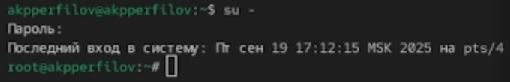
\includegraphics[width=0.7\linewidth,height=\textheight,keepaspectratio]{image/1.jpg}

}

\caption{Получение полномочий администратора, ввод трёх команд,
остановка процесса, установка выполнения задания 3 в фоновом режиме,
просмотр изменений в статусе заданий}

\end{figure}%

Для перемещения задания 1 на передний план введём fg 1, далее введём
Ctrl+ c, чтобы отменить задание 1. С помощью команды jobs посмотрим
изменения в статусе заданий и проделаем то же самое для отмены заданий 2
и 3

\begin{figure}

{\centering 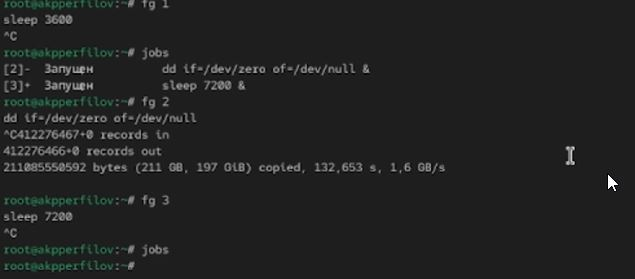
\includegraphics[width=0.7\linewidth,height=\textheight,keepaspectratio]{image/2(1).jpg}

}

\caption{Перемещение заданий на передний план и их последующая отмена.}

\end{figure}%

Теперь откроем второй терминал и под учётной записью пользователя введём
в нём: dd if=/dev/zero of=/dev/null \&. После введём exit, чтобы закрыть
второй терминал

\begin{figure}

{\centering 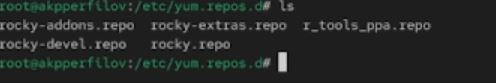
\includegraphics[width=0.7\linewidth,height=\textheight,keepaspectratio]{image/3.jpg}

}

\caption{Ввод команды и закрытие терминала.}

\end{figure}%

На другом терминале под учётной записью своего пользователя запустим
top. Мы увидим, что задание dd всё ещё запущено. Для выхода из top
используем q и вновь запусткаем top, в нём используем k, чтобы убить
задание dd. После этого выйдем из top

\begin{figure}

{\centering 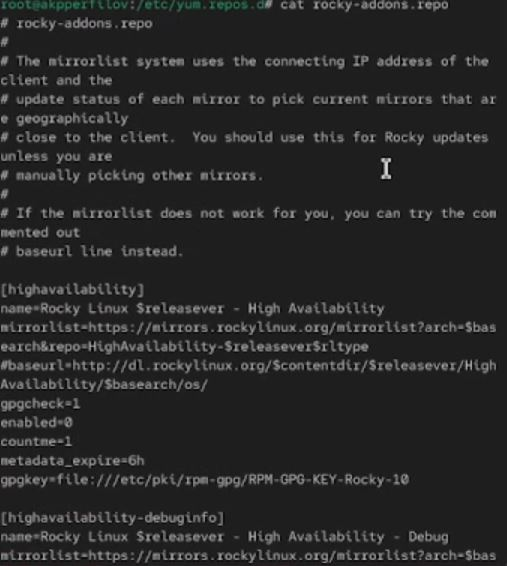
\includegraphics[width=0.7\linewidth,height=\textheight,keepaspectratio]{image/4.jpg}

}

\caption{Убийство задания dd в top.}

\end{figure}%

\section{Управление
процессами}\label{ux443ux43fux440ux430ux432ux43bux435ux43dux438ux435-ux43fux440ux43eux446ux435ux441ux441ux430ux43cux438}

Получим полномочия администратора su - и введём следующие команды:

dd if=/dev/zero of=/dev/null \& dd if=/dev/zero of=/dev/null \& dd
if=/dev/zero of=/dev/null \&

После чего введём ps aux \textbar{} grep dd, которое показывает все
строки, в которых есть буквы dd. Запущенные процессы dd идут последними.
Используем PID первого процесса dd, чтобы изменить приоритет (renice -n
5)

\begin{figure}

{\centering 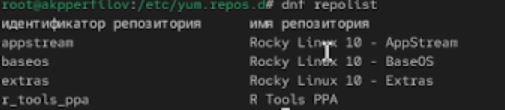
\includegraphics[width=0.7\linewidth,height=\textheight,keepaspectratio]{image/5.PNG}

}

\caption{Получение полномочий администратора, ввод команд. Просмотр всех
строк, в которых есть dd. Изменение приоритета.}

\end{figure}%

Введём ps fax \textbar{} grep -B5 dd. Параметр -B5 показывает
соответствующие запросу строки, включая пять строк до этого. Поскольку
ps fax показывает иерархию отношений между процессами, мы также видим
оболочку, из которой были запущены все процессы dd, и её PID

\begin{figure}

{\centering 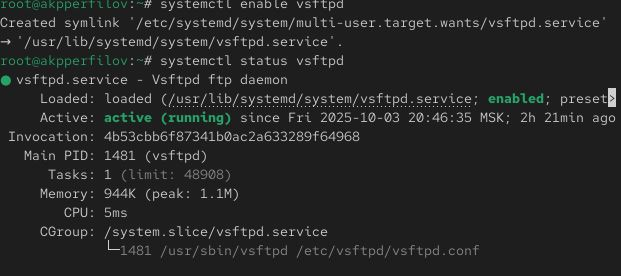
\includegraphics[width=0.7\linewidth,height=\textheight,keepaspectratio]{image/6.jpg}

}

\caption{Просмотр иерархии отношений между процессами.}

\end{figure}%

Теперь найдём PID корневой оболочки, из которой были запущены процессы
dd, и введём kill -9 (указав PID оболочки). Мы увидим, что наша корневая
оболочка закрылась, а вместе с ней и все процессы dd (остановка
родительского процесса --- простой и удобный способ остановить все его
дочерние процессы)

\begin{figure}

{\centering 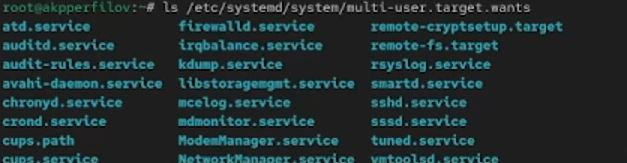
\includegraphics[width=0.7\linewidth,height=\textheight,keepaspectratio]{image/7.jpg}

}

\caption{Закрытие корневой оболочки.}

\end{figure}%

\chapter{Выполнение заданий для самостоятельной
работы}\label{ux432ux44bux43fux43eux43bux43dux435ux43dux438ux435-ux437ux430ux434ux430ux43dux438ux439-ux434ux43bux44f-ux441ux430ux43cux43eux441ux442ux43eux44fux442ux435ux43bux44cux43dux43eux439-ux440ux430ux431ux43eux442ux44b}

\section{Самостоятельная работа (задание
1)}\label{ux441ux430ux43cux43eux441ux442ux43eux44fux442ux435ux43bux44cux43dux430ux44f-ux440ux430ux431ux43eux442ux430-ux437ux430ux434ux430ux43dux438ux435-1}

Получим полномочия администратора su -- и запустим команду dd
if=/dev/zero of=/dev/null \& трижды как фоновое задание. Затем увеличим
приоритет первой команды, используя значение приоритета −5, после чего
изменим приоритет того же процесса ещё раз, но используем на этот раз
значение −15 (мы можем менять приоритет команды от -20 (самый высокий
приоритет) до 19 (самый низкий приоритет)). Завершим все процессы dd,
которые мы запустили командой: killall dd

\begin{figure}

{\centering 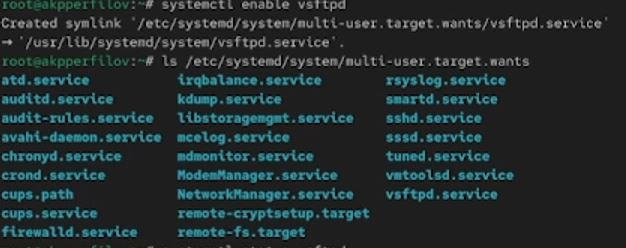
\includegraphics[width=0.7\linewidth,height=\textheight,keepaspectratio]{image/8.jpg}

}

\caption{Получение полномочий администратора, запуск команды трижды как
фоновое задание.}

\end{figure}%

\begin{figure}

{\centering 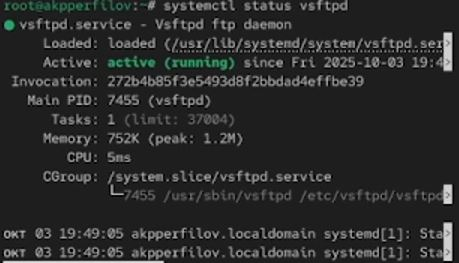
\includegraphics[width=0.7\linewidth,height=\textheight,keepaspectratio]{image/9.jpg}

}

\caption{Увеличение приоритета первой команды.}

\end{figure}%

\begin{figure}

{\centering 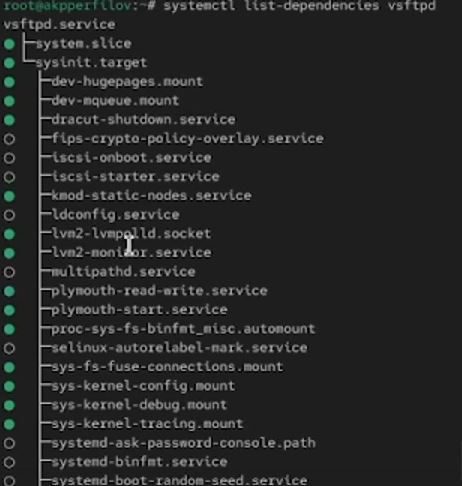
\includegraphics[width=0.7\linewidth,height=\textheight,keepaspectratio]{image/10.jpg}

}

\caption{Увеличение приоритета первой команды.}

\end{figure}%

\begin{figure}

{\centering 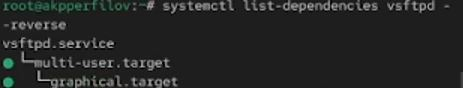
\includegraphics[width=0.7\linewidth,height=\textheight,keepaspectratio]{image/11.jpg}

}

\caption{Завершение всех процессов.}

\end{figure}%

\section{Самостоятельная работа (задание
2)}\label{ux441ux430ux43cux43eux441ux442ux43eux44fux442ux435ux43bux44cux43dux430ux44f-ux440ux430ux431ux43eux442ux430-ux437ux430ux434ux430ux43dux438ux435-2}

Получим полномочия администратора su -- и запустим программу yes в
фоновом режиме с подавлением потока вывода (yes \textgreater{} /dev/null
\&), далее запустим программу yes на переднем плане с подавлением потока
вывода и приостановим выполнение программы. Заново запустим программу
yes с теми же параметрами, затем завершим её выполнение. Повторим
действия, но уже запустим программу yes на переднем плане без подавления
потока вывода (yes \textgreater{} /dev/null). Также приостановим
выполнение программы и заново запустим программу yes с теми же
параметрами, затем завершим её выполнение. Проверим состояния заданий,
воспользовавшись командой jobs. Далее переведём процесс, который у нас
выполняется в фоновом режиме, на передний план, затем остановим его (fg
1, после чего Ctrl+c). Переведём 3 процесс с подавлением потока вывода в
фоновый режим (bg 3) и проверим состояния заданий, воспользовавшись
командой jobs. Обратим внимание, что процесс стал выполняющимся
(Running) в фоновом режиме. Запустим процесс в фоновом режиме таким
образом, чтобы он продолжил свою работу даже после отключения от
терминала (nohup yes \textgreater{} /dev/null \&). Закроем окно и заново
запустим консоль. Убедимся, что процесс продолжил свою работу

\begin{figure}

{\centering 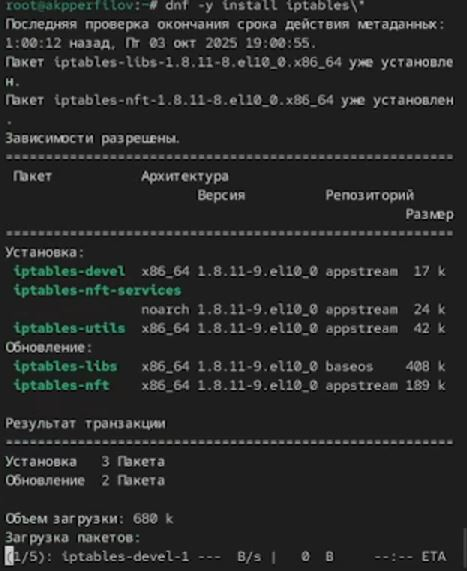
\includegraphics[width=0.7\linewidth,height=\textheight,keepaspectratio]{image/12.jpg}

}

\caption{Получение полномочий администратора. Запуск программы yes в
фоновом режиме с подавлением потока вывода. Запуск программы yes на
переднем плане без подавления потока вывода. Перевод процесса на
передний план и его остановка. Перевод процесса в фоновый режим.
Проверка состояния заданий. Запуск процесса в фоновом режиме с
условиями.}

\end{figure}%

Сейчас получим информацию о запущенных в операционной системе процессах
с помощью утилиты top

\begin{figure}

{\centering 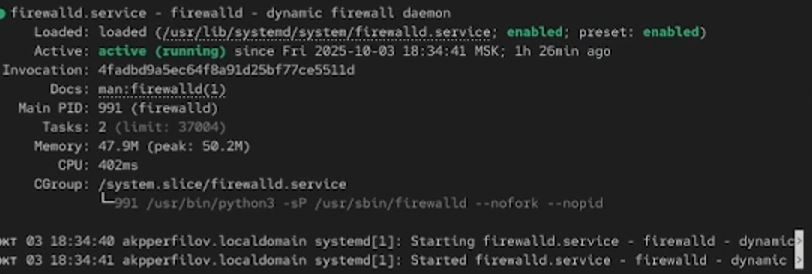
\includegraphics[width=0.7\linewidth,height=\textheight,keepaspectratio]{image/13.jpg}

}

\caption{Получение информации о запущенных в операционной системе
процессах.}

\end{figure}%

Запустим ещё три программы yes в фоновом режиме с подавлением потока
вывода (yes \textgreater{} /dev/null \&). Убьём два процесса: для одного
используем его PID (kill -9), а для другого --- его идентификатор
конкретного задания (fg 2 и Ctrl+c). Попробуем послать сигнал 1 (SIGHUP)
процессу, запущенному с помощью nohup (kill -1), и обычному процессу
(kill -1)

\begin{figure}

{\centering 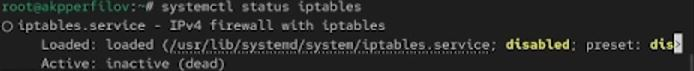
\includegraphics[width=0.7\linewidth,height=\textheight,keepaspectratio]{image/14.jpg}

}

\caption{Запуск трёх программ yes в фоновом режиме с подавлением потока
вывода, убийство двух процессов, попытка послать сигнал 1 (SIGHUP).}

\end{figure}%

Запустим ещё несколько программ yes в фоновом режиме с подавлением
потока вывода (yes \textgreater{} /dev/null \&) и завершим их работу
одновременно, используя команду killall yes

\begin{figure}

{\centering 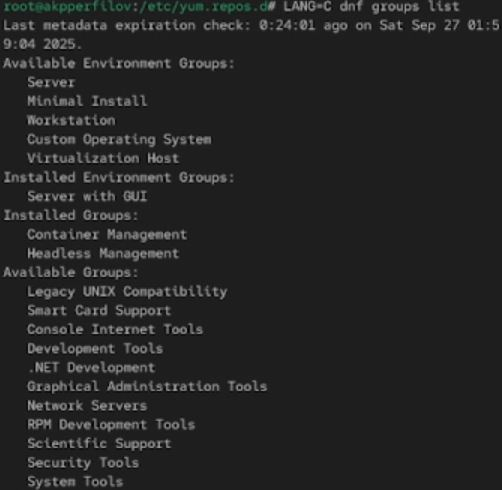
\includegraphics[width=0.7\linewidth,height=\textheight,keepaspectratio]{image/15.jpg}

}

\caption{Запуск программ yes в фоновом режиме с подавлением потока
вывода и одновременное завершение их работы.}

\end{figure}%

После чего запустим программу yes в фоновом режиме с подавлением потока
вывода (yes \textgreater{} /dev/null \&). Используя утилиту nice (nice
-n 15 yes), запустим программу yes с теми же параметрами и с
приоритетом, большим на 5. Сравним абсолютные и относительные приоритеты
у этих двух процессов (ps -l \textbar{} grep yes). Используя утилиту
renice, изменим приоритет у одного из потоков yes таким образом, чтобы у
обоих потоков приоритеты были равны (renice -n 15) (рис.

\begin{figure}

{\centering 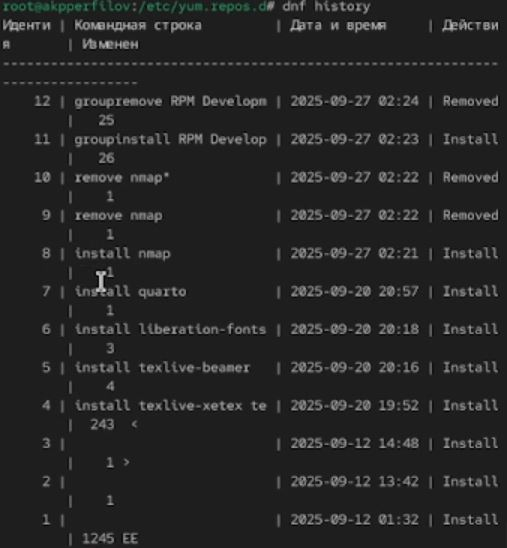
\includegraphics[width=0.7\linewidth,height=\textheight,keepaspectratio]{image/16.jpg}

}

\caption{Запуск программы yes в фоновом режиме с подавлением потока
вывода. Запуск программы yes с теми же параметрами и с приоритетом,
большим на 5. Сравнение абсолютных и относительных приоритетов,
изменение приоритета.}

\end{figure}%

\chapter{Ответы на контрольные
вопросы}\label{ux43eux442ux432ux435ux442ux44b-ux43dux430-ux43aux43eux43dux442ux440ux43eux43bux44cux43dux44bux435-ux432ux43eux43fux440ux43eux441ux44b}

\begin{enumerate}
\def\labelenumi{\arabic{enumi}.}
\tightlist
\item
  Какая команда даёт обзор всех текущих заданий оболочки?
\end{enumerate}

jobs.

\begin{enumerate}
\def\labelenumi{\arabic{enumi}.}
\setcounter{enumi}{1}
\tightlist
\item
  Как остановить текущее задание оболочки, чтобы продолжить его
  выполнение в фоновом режиме?
\end{enumerate}

bg номер\_задания

\begin{enumerate}
\def\labelenumi{\arabic{enumi}.}
\setcounter{enumi}{2}
\tightlist
\item
  Какую комбинацию клавиш можно использовать для отмены текущего задания
  оболочки?
\end{enumerate}

Ctrl+c.

\begin{enumerate}
\def\labelenumi{\arabic{enumi}.}
\setcounter{enumi}{3}
\tightlist
\item
  Необходимо отменить одно из начатых заданий. Доступ к оболочке, в
  которой в данный момент работает пользователь, невозможен. Что можно
  сделать, чтобы отменить задание?
\end{enumerate}

Внутри top использовать k, чтобы убить задание.

\begin{enumerate}
\def\labelenumi{\arabic{enumi}.}
\setcounter{enumi}{4}
\tightlist
\item
  Какая команда используется для отображения отношений между
  родительскими и дочерними процессами?
\end{enumerate}

ps fax.

\begin{enumerate}
\def\labelenumi{\arabic{enumi}.}
\setcounter{enumi}{5}
\tightlist
\item
  Какая команда позволит изменить приоритет процесса с идентификатором
  1234 на более высокий?
\end{enumerate}

renice -n приоритет\_процесса .

\begin{enumerate}
\def\labelenumi{\arabic{enumi}.}
\setcounter{enumi}{6}
\tightlist
\item
  В системе в настоящее время запущено 20 процессов dd. Как проще всего
  остановить их все сразу?
\end{enumerate}

killall dd.

\begin{enumerate}
\def\labelenumi{\arabic{enumi}.}
\setcounter{enumi}{7}
\tightlist
\item
  Какая команда позволяет остановить команду с именем mycommand?
\end{enumerate}

Сначала узнаем PID процесса mycommand -ps aux \textbar{} grep mycommand
далее команда kill -9 .

\begin{enumerate}
\def\labelenumi{\arabic{enumi}.}
\setcounter{enumi}{8}
\tightlist
\item
  Какая команда используется в top, чтобы убить процесс?
\end{enumerate}

\begin{enumerate}
\def\labelenumi{\alph{enumi}.}
\setcounter{enumi}{10}
\tightlist
\item
\end{enumerate}

\begin{enumerate}
\def\labelenumi{\arabic{enumi}.}
\setcounter{enumi}{9}
\tightlist
\item
  Как запустить команду с достаточно высоким приоритетом, не рискуя, что
  не хватит ресурсов для других процессов?
\end{enumerate}

Запустить команду в фоновом режиме.

\chapter{Выводы}\label{ux432ux44bux432ux43eux434ux44b}

В ходе выполнения лабораторной работы были получены навыки управления
процессами операционной системы.


\printbibliography



\end{document}
